\section{OMNeT++}\label{sec:omnetpp}

\omnetpp{} is an extensible, modular, component-based C++ simulation library
and framework, primarily for building network simulators
\cite{omnetpp-simulation-manual}. Publicly available under the Academic Public
License, it can be freely used for non-profit purposes. \omnetpp{} is tailored
for large-scale simulations with hierarchical models, supporting the
visualization, debugging and customization of simulation models, and includes
tools for analyzing simulation results \cite{omnetpp}.

The framework includes a topology description language called NED, which allows
users to define model structure and network topologies using object-oriented
features like inheritance and interfaces.

Starting from the user-provided C++ model, \omnetpp{} generates an executable
containing both the simulation model and the \omnetpp{}'s simulation kernel. An
overview of the \omnetpp{} architecture is shown in
\figref{fig:omnetpp-architecture}.

\begin{figure}[tbhp]
	\centering
	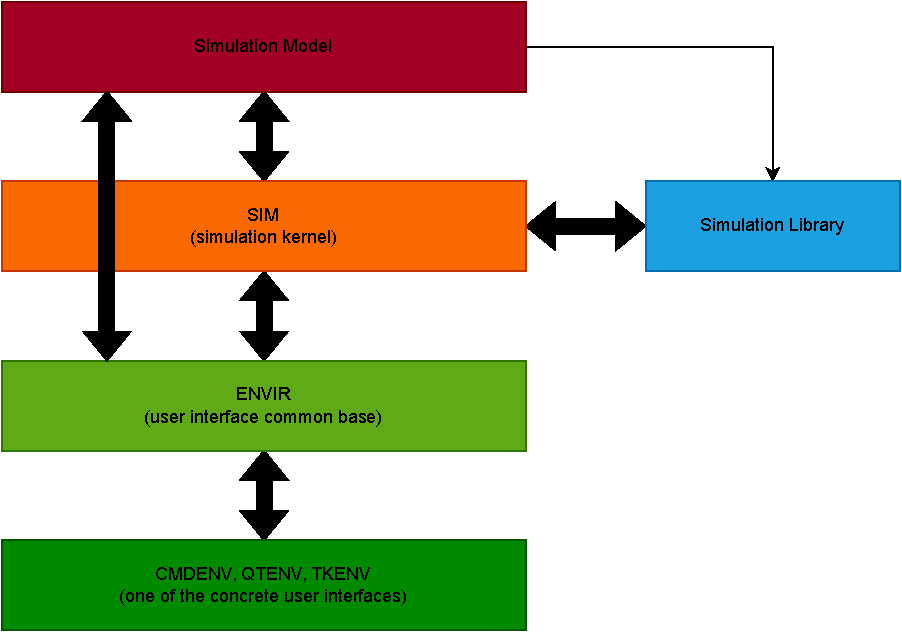
\includegraphics[width=0.5\textwidth]{opparch}
	\caption{OMNeT++ architecture. The Simulation Model builds on classes
	from the Simulation Library to implement model-specific functionality.
	The Simulation Kernel manages simulation execution and event
	scheduling. Different user interfaces are available to monitor and
	control the execution.}\label{fig:omnetpp-architecture}
\end{figure}

An \omnetpp{} simulation consists of a network, which is a collection of
modules connected by channels, and a configuration, which specifies parameter
values to guide the simulation's trajectory. Modules are categorized as either
\emph{simple} or \emph{compound}:
\begin{itemize}
	\item \textbf{Simple modules} are the basic building blocks,
		encapsulating the simulation's logic;
	\item \textbf{Compound modules} serve as containers to group simple
		modules, but they do not have logic themselves.
\end{itemize}

Simple modules exchange \emph{messages} through \emph{gates}. These messages,
which are the actual \emph{events} of the simulation, are scheduled for
delivery at specific times, and the simulation kernel ensures their timely
delivery to the appropriate module. Alternatively, when direct interaction is
preferred over message-based communication, modules can invoke each other's
methods via \emph{Direct Method Calls} (DMCs).

Messages themselves are standard C++ classes, capable of containing fields and
methods. \omnetpp{} simplifies the creation of message types with its message
definition language, which is subsequently compiled into C++ code.

The logic of simple modules is implemented in C++ by inheriting from the
\code{cSimpleModule} class. Users can define the behavior of a module by
overriding the following methods:
\begin{itemize}
	\item \code{initialize()}: sets up the module at the start of the
		simulation, called after the class constructor;
	\item \code{handleMessage()}: specifies how the module processes
		incoming messages;
	\item \code{finish()}: finalizes operations and collects statistics at
		the end of the simulation, prior to the destructor being
		called.
\end{itemize}

The structure of an \omnetpp{} network is illustrated in
\figref{fig:omnetpp-network}. Blue boxes represent gates, which connect modules
via channels.

\begin{figure}[tbhp]
	\centering
	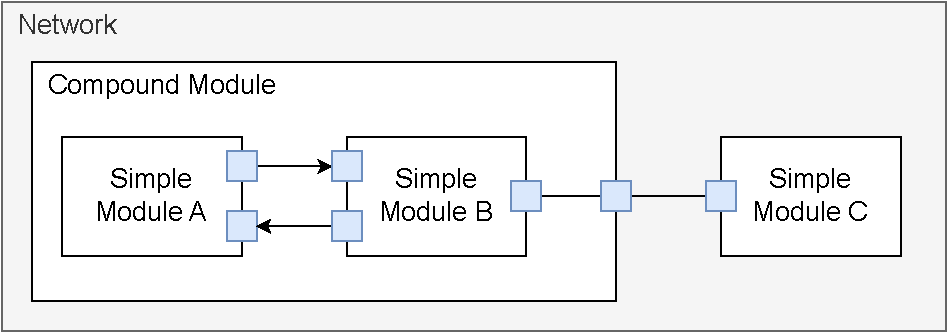
\includegraphics[width=0.5\textwidth]{oppnetwork}
	\caption{Structure of an \omnetpp{}
	network.}\label{fig:omnetpp-network}
\end{figure}

\omnetpp{} offers a powerful mechanism for gathering statistics. Simple modules
can emit signals, which are collected and processed according to instructions
specified in NED files. This feature facilitates in-depth analysis of
simulation behavior.

As discussed in \chref{ch:intro}, the goal of this work is to create a Bitcoin
simulator capable of running large-scale simulations within reasonable
timeframes. Given the importance of performance, the use of compiled native
code was imperative. The combination of C++ and \omnetpp{} was chosen as it
provides both high execution efficiency and extensive modeling capabilities.

Further information on \omnetpp{} is available on the official website
\cite{omnetpp-website}, in the simulation manual
\cite{omnetpp-simulation-manual}, and in the paper of its authors
\cite{omnetpp}.
